\section{Централизованный подход}
Назначение верхнеуровневой системы управления микрогридом~--- экономически оптимальное распределение мощности между генерирующим и аккумулирующим оборудованием и нагрузкой (задачи \textit{unit commitment} или \textit{optimal dispatch}).

Из этой задачи отдельно можно выделить задачу управления режимом работы оборудования: часто приведение устройства в рабочий режим связано с затратами энергии и расходованием ресурса оборудования.
Например, запуск дизель-генератора требует его предварительного прогрева, а условия его эксплуатации не допускают частых включений-выключений из-за износа \cite{bleijs1993wear}, поэтому, будучи включен в отсутствии нагрузки, он будет вынужден работать некоторое время на холостом ходу.
Топливные элементы и электролизные установки так же требуют предварительного прогрева и времени для выхода на режим. 
Поэтому будем отдельно рассматривать \textit{задачу выбора уставок} мощности и задачу выбора режима работы оборудования~--- \textit{задачу планирования}.
%  \textit{откладываемой} нагрузкой, т. е. нагрузкой, удовлетворение которой может быть сдвинуто во времени, например, нагрузка на обогрев помещения 

Структура этого раздела следующая:
в начале мы сформулируем  задачу планирования (подразделы \ref{sec:system_definition}--\ref{sec:planning_math}),
и приведём результаты численных экспериментов (подраздел \ref{sec:planning_numeric}).
Затем покажем, что задача выбора уставок может быть сведена к практически такой же математической формулировке.
Завершает раздел обзор более продвинутых подходов к задаче планирования.
Результаты численных экспериментов будут приведены сразу для децентрализованной системы управления в разделе \ref{sec:decentralized}.

Цель этого раздела~---  введение наиболее простой модели, отражающей основные особенности изолированной энергосистемы, формулировка и имплементация простой системы управления в виде оптимизационной задачи и интерпретация полученных результатов.
Хотя возможно построение простых систем управления, имеющих вид цепочек условных операторов \cite{Aziz2019}, дизайн таких систем управления предполагает, что выполнены определённые соотношения между параметрами компонентов управляемой системы, поэтому они не универсальны и являются частными решениями универсальных оптимизационных задач управления энергосистемой.
Ещё одним плюсом описания системы управления в виде оптимизационной задачи является возможность добавления ограничений и учёта новых факторов без существенного изменения кода или даже в рамках одной математической формулировки.

Содержание этого раздела близко к содержанию статьи Barley, Winn \cite{Barley1996}, в которой проводится сравнительный анализ эвристических стратегий управления микрогридом. 
Общий подход к задаче, предложенный в статье Barley, Winn, используется в одном из наиболее популярных программных пакетов для оптимального дизайна микрогридов Homer Pro, часто применяемом для валидации результатов в научных работах \cite{Berendes2018, Aziz2019, Petersen2018, Olatomiwa2016}.

% \subsection{Постановка задачи}
% \label{sec:planning_problem}
\subsection{Описание компонентов физической системы}
\label{sec:system_definition}

Решается задача оптимального управления автономной энергетической системой.\\
Рассматриваемая система включает неконтроллируемый источник ``бесплатной'' возобновляемой энергии  (ветрогенератор или фотовольтаическая солнечная установка), дизель-генератор, накопитель энергии и постоянную неуправляемую нагрузку.
В качестве базового варианта накопителя энергии рассматривается литий-ионный электрохимический аккумулятор, ставший вариантом по-умолчанию для установки в микрогридах за счёт оптимального соотношения между мощностью и энергетической ёмкостью, хорошему ресурсу и способностью практически мгновенно изменять величину потребляемой/выдаваемой мощности.
С соответствующими допущениями написанное в этом разделе можно применить и к другим типам накопителей. 

Пренебрегая зависимостью интенсивности износа аккумуляторной батареи от глубины заряда/разряда и величины токов, считаем, что стоимость использования батареи определяется её капитальной стоимостью и ресурсом, равным количеству электрической энергии, которая может пройти через батарею до того, как батарею необходимо будет заменить.
Таким образом, стоимость использования батареи определяется по формуле \cite{bwc}:


\begin{equation}\label{f:cb}
c_b(P) \left[\frac{\$}{h} \right] = 
a_b \cdot P,
\end{equation}
\begin{equation}\label{f:ab}
a_b \left[ \frac{\$}{kW\cdot h} \right] =
\frac{\text{batteryPrice}}{\text{batteryCapacity} \cdot \text{batteryMaxCycles} 
\cdot \sqrt{\eta}} ,
\end{equation}
здесь batteryPrice~[\$]~--- капитальная стоимость батареи,\\
batteryCapacity~[$kW\cdot h$]~--- энергетическая ёмкость батареи,\\
batteryMaxCycles~--- число полных циклов заряда-разряда до замены батареи,\\
$\eta$~--- энергетический КПД цикла заряда-разряда.

    
Для включенного дизельного генератора зависимость расхода топлива от мощности:
\begin{equation}
 \text{fuelConsumption} (P) = \text{fuelIntercept} + \text{fuelSlope} \cdot P.
\end{equation}

Тогда стоимость использования дизель-генератора:

\begin{equation}\label{f:cg}
c_g(P) \left[\frac{\$}{h} \right] = b_g + a_g \cdot P,
\end{equation}


\begin{equation}\label{f:bg}
b_g \left[\frac{\$}{h} \right] = 
\text{fuelIntercept} \cdot \text{fuelCost} + \text{maintainanceCost} +
\frac{\text{gensetPrice}}{\text{gensetResource}},
\end{equation}

\begin{equation}\label{f:ag}
a_g \left[ \frac{\$}{kW\cdot h} \right] = 
\text{fuelSlope} \cdot \text{fuelCost}.
\end{equation}
Здесь maintainanceCost~[\$ / моточас]~--- стоимость обслуживания,\\ 
gensetPrice~[\$]~--- капитальная стоимость генераторной установки,\\
gensetResource~[моточас]~--- количество моточасов до замены.

Здесь предполагается, что ресурс дизель-генератора, в отличии от ресурса электрохимического аккумулятора, зависит от количества часов в работе, но не зависит от мощности.
Действительно, основной показатель надёжности, предоставляемый производителями дизель-генераторов~--- это время наработки на отказ   (ГОСТ Р 53176-2008). 
Кроме того, аналогичная электрохимическим накопителям модель деградации, в которой ресурс зависит от выработанной энергии не применим для дизель-генераторов, так как длительная эксплуатация с мощностью, меньшей 40-50\% от номинальной приводит к дополнительному износу дизель-генератора \cite{bleijs1993wear}.


Соответствующие экономической модели графики изображены на Рис \ref{fig:bgcost}.

\subsection{Стратегии для задачи планирования}
\label{sec:strategies}

Простейшим подходом к задаче поиска экономически оптимального на всём периоде эксплуатации системы управления с соблюдением баланса мощности при отсутствии информации о будущей ветрогенерации является применение эвристических правил-стратегий.

Для простоты будем рассматривать систему с одним дизель-генератором. 
Обобщение на случай нескольких дизель-генераторов не составляет труда.

Для определённости будем считать, что минимальный приемлемый период между включениями-выключениями дизель-генератора равен одному часу.
Тогда задача планирования состоит в том, чтобы решить, должен ли дизель-генератор быть включен в течении следующего часа, или нет.
Чтобы принять решение, будем использовать прогнозное значение средней мощности ветрогенерации.
\cite{foley2012current}


% Требуется найти оптимальные с точки зрения экономического критерия уставки мощности для дизель-генератора и батареи с условием поддержания баланса мощности (здесь и далее \textit{мощность} означает \textit{активная мощность}) в системе в течении следующего после принятия решения часа \textit{(задача планирования)}.
% На ближайший час значение мощности ветрогенерации считается постоянным и известным.

В пакете Homer Pro, по умолчанию используются две такие стратегии: \textit{Load Following (LF)} \cite{lf} и \textit{Cycle Charging (CC)} \cite{cc}.

В стратегии LF уставка генератору выбирается такой, чтобы обеспечить баланс мощности, не производя дополнительной энергии для зарядки батареи или, при наличии, обслуживания откладываемой нагрузки (defferable load).
То есть согласно стратегии LF выбирается управление, наиболее дешёвым образом обеспечивающее баланс мощности на ближайший квант времени планирования (локально-оптимальное).

В стратегиях $CC$ допускается заряжать аккумулятор от дизель-генератора не смотря на дополнительный расход ресурса батареи и потери энергии в цикле заряда-разряда, так как это позволяет \cite{Barley1996}:
\begin{enumerate}
    \item  эксплуатировать дизель-генератор в точке его максимального КПД,
    \item уменьшить количество запусков/выключений дизель-генератора.
\end{enumerate}

Среди нескольких похожих способов-правил формулировки стратегии СС мы остановимся на следующей: сначала находится управление по стратегии LF, после чего ненулевые уставки генераторов повышаются до их номинальной мощности или до максимальной мощности, которую готовы принять аккумуляторная батарея и нагрузка.

Хотя оптимальность той или иной стратегии зависит от многих факторов, таких как коэффициенты, соответствующие техническим и экономическим параметрам оборудования \cite[177]{Barley1996}, считается \cite{homer_control}, что стратегия CC лучше подходит для систем с незначительной или нулевой долей возобновляемой энергии, а LF~--- для систем, преимущественно обеспечиваемых ВИЭ.

Также в литературе \cite[10]{Aziz2019} встречается несколько иная, чисто оптимизационная формулировка стратегии CC,  будем обозначать её CC2. 
Здесь, как и в стратегии LF ищется локально-оптимальное управление, но в экономический критерий оптимальности вводится дополнительная величина, \textit{стоимость энергии батареи} \cite{bec}:
\begin{equation}\label{f:bec}
    a_{be} = \frac{C_{cc}}{E_{bc}},
\end{equation}
где $C_{cc}$ --- расходы на энергию, произведённую специально для того, чтобы зарядить батарею (в процессе Cycle Charging);\\
$E_{bc}$ --- суммарное количество энергии, переданное батарее.
И в ограничения добавляется условие, что, как и в стратегии $CC$ мощность генератора должна быть либо нулевой, либо быть равной минимуму из его номинальной мощности и максимальной мощности, которую готова принять система.

Зарядка батареи от ветрогенератора считается бесплатной, поэтому в числителе учитываются только расходы от использования дизель-генератора для зарядки батареи.
При оптимизации считается, что при разрядке батареи система теряет деньги, равные стоимости энергии батареи, умноженной на энергию разряда, а при зарядке~--- получает.
То есть если батарея часто заряжается от ветрогенератора, стоимость энергии батареи мала и системе не выгодно заряжать батарею от генератора, а разряжать батарею, наоборот, не затратно.
Если же ветрогенерации мало, стоимость энергии батареи высока и системе выгодно увеличивать мощность дизель-генератора для зарядки батареи.

Для корректной работы алгоритма необходимо разумно инициализировать стоимость энергии батареи, пока батарея не получала энергию и пользоваться формулой (\ref{f:bec}) невозможно.
До этого момента полагаем $a_{be} = a_b / 2$.

\subsection{Математические формулировки для задачи планирования}
\label{sec:planning_math}
Теперь сформулируем задачи поиска управления по стратегиям LF, CC, CC2 в виде задач смешанного целочисленно-линейного программирования~(MILP).

\paragraph{LF}
\label{par:lf}
\begin{equation}\label{f:lf}
\begin{split}
\vspace{-4mm}
&f = -\eps z_+ - a_b z_- 
+ b_g x + a_g y
\rightarrow \min\limits_{(x, y, z_+, z_-) \in \{0,1\} \times \R^3 }\\
\text{s.t. }& y + P_{wind} \geq P_{load} + z_+ + z_-\\
&y \leq x \cdot P_{genset~max}\\
&0 \leq y \\
&0 \leq z_+ \leq P_{battery~ch~max} \\
&-P_{battery~disch~max} \leq z_- \leq 0 \\
\end{split}
\end{equation}
Здесь $x$ --- включён ли генератор,\\
$y$ --- мощность генератора,\\
$z_+$ --- мощность заряда батареи,\\
$z_-$ --- мощность разряда батареи со знаком минус,\\
$\eps$ --- достаточно малое число --- поощрение за заряд батареи,\\
$P_{battery~ch~max},~P_{battery~disch~max}$~--- максимальные доступные на следующий час мощности заряда и разряда батареи, посчитанные с учётом её текущего заряда.

Уставки мощности генератору и батарее (разряду соответствует отрицательная уставка) равны $y$ и $z_+ + z_-$ соответственно.

Поскольку в стратегию LF не заложена ценность энергии батареи, но LF подразумевает, что вся избыточная энергия ветрогенерации по возможности поглащается батареей, в критерий оптимальности вводится дополнительное слагаемое $-\eps z_+$, а плата за износ батареи при её заряде переносится в плату за разряд батареи.


\paragraph{CC}
Пусть $(x, y, z_+, z_-)$ --- решение (\ref{f:lf}).\\
Пусть $P_{gm} := \min(P_{genset~max}, P_{load}- P_{wind} + P_{battery~ch~max})$.\\
Тогда уставки генератору и батарее равны соответственно $P_{gm}x$ и $z_+ + z_- + P_{gm}x - y$.

\paragraph{CC2}

\begin{equation}\label{f:cc2}
\begin{split}
&f = \frac{a_b}{2}(z_+ - z_-) - a_{be}(z_+ + z_-)
+ (b_g  + a_g P_{gm}) x
\rightarrow \min\limits_{(x, z_+, z_-) \in \{0,1\} \times \R^2 }\\
\text{s.t. }& y + P_{wind} \geq P_{load} + z_+ + z_-\\
&0 \leq z_+ \leq P_{battery~ch~max} \\
&-P_{battery~disch~max} \leq z_- \leq 0 \\
\end{split}
\end{equation}


Здесь плата за износ батареи разделена поровну между зарядом и разрядом.
Уставки генератора и батареи равны $P_{gm}x$ и $z_+ + z_-$.

\medskip
Для всех этих оптимизационных задач точное решение мгновенно вычисляется дефолтным солвером PuLP.

\subsection{Численные эксперименты со стратегиями для задачи планирования}
\label{sec:planning_numeric}

Три описанные выше стратегии были использованы для управления системой на 134-часовом периоде и оценены по критериям суммарной экономической эффективности, количеству использованного топлива,  ресурса батареи и дизель-генератора.
В качестве прогнозного среднего значения мощности ветрогенерации использовалось реальное среднее значение мощности ветрогенерации за следующий час. 
Код симуляции доступен по \href{https://github.com/niquepolice/electro/blob/03f136b13663806bfba4a4ce973f524558564363/milp.ipynb}{ссылке}.

В качестве параметров системы были взяты значения:\\
$\text{gensetPrice} = \dfrac{2.5e6}{75}\$$\\
$\text{gensetResource} = 15000h$\\
$\text{maintainanceCost} = 3\$/h$\\
$\text{fuelIntercept} = 2L/h$\\
$\text{fuelSlope} = (28-2)/100 L/kWh$\\
$\text{fuelPrice} = \dfrac{64}{75}\$/L$\\
% $\text{batteryPrice} = \frac{64}{75}\$/L$
$\text{batteryMaxCycles} = 3000$\\
$\text{batteryCapacity} = 100kWh$\\
$\eta = 1$ \\
$P_{genset max} = 100kW$ \\
$P_{battery max} = 3\text{batteryCapacity} / h$

Для удельной (по ёмкости) стоимости батареи протестированы два значения, соответствующие двум разным режимам работы системы: когда $a_b > a_g$ ($1000\$/kWh$) и $a_b < a_g$ ($400\$/kWh$).
Графики стоимости использования батареи и генератора двух таких режимов показаны на Рис~\ref{fig:bgcost}.


\begin{figure}[h]
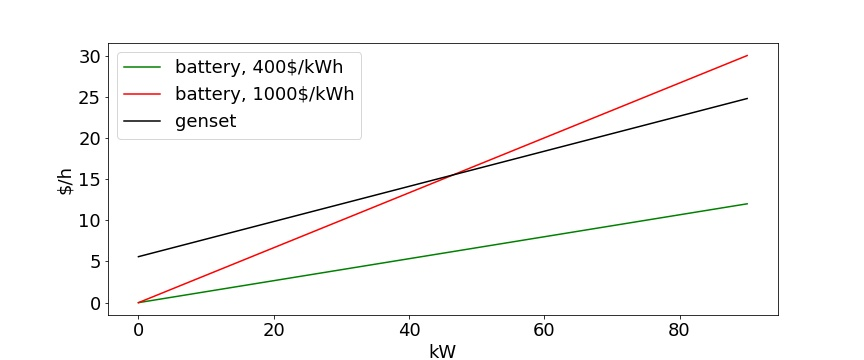
\includegraphics[scale=0.5]{energy_cost.jpeg}
\caption{Стоимость использования батареи и дизель-генератора}
\centering
\label{fig:bgcost}
\end{figure}

\medskip

Для нагрузки так же протестированы два значения: 70кВт и 30кВт.

Результаты представлены в Таблице \ref{t:res} и на Рисунках \ref{fig:res_70_400}, \ref{fig:res_70_1000} и \ref{fig:res_30} в Приложениях.
По результатам видно, что стратегии CC и СС2 незначительно отличаются при большой нагрузке и абсолютно эквивалентны при малой, поэтому для нагрузки 30кВт приведены только графики по CC. 
При дешёвой батарее лучшие результаты показывают CC и СС2, а при дорогой~--- LF, причем при малой нагрузке и дешёвой батарее разница существенна, а при остальных параметрах выражена менее явно.
Во всех случаях LF экономнее по отношению к ресурсу батареи, а СС~--- по отношению к топливу и моточасам.


\begin{table}[h]
\caption{Результаты применения стратегий на модели}
\label{t:res}
\begin{tabular}{{|p{1.9cm}|p{1.8cm}|p{2cm}|p{2cm}|p{2cm}|p{2cm}|p{2cm}|  }}
\hline
Стратегия & Нагрузка, кВт & Стоимость аккумулятора, \$/кВт ч & Остаток ресурса батареи, \% & Расход топлива, л & Количество часов работы дизель-генератора & Суммарные расходы, \$ \\
\hline
lf       & 70   & 400          & 99.89                & 1667             & 100       & 2022       \\
cc       & 70   & 400          & 99.18                & 1567             & 56        & 1974       \\
cc2      & 70   & 400          & 99.55                & 1645             & 72        & 1985       \\
lf       & 70   & 1000         & 99.9                 & 1660             & 97        & 2058       \\
cc       & 70   & 1000         & 99.69                & 1654             & 79        & 2154       \\
cc2      & 70   & 1000         & 99.82                & 1714             & 89        & 2136       \\
lf       & 30   & 400          & 99.9                 & 549              & 61        & 849        \\
cc       & 30   & 400          & 99.55                & 447              & 16        & 650        \\
cc2      & 30   & 400          & 99.55                & 447              & 16        & 650        \\
lf       & 30   & 1000         & 99.9                 & 542              & 58        & 882        \\
cc       & 30   & 1000         & 99.55                & 447              & 16        & 918        \\
cc2      & 30   & 1000         & 99.55                & 447              & 16        & 918      \\ 
\hline
\end{tabular}
\end{table}

\subsection{Задача выбора уставок мощности}
\label{sec:references}
    Двигаясь дальше, необходимо уточнить модель и постановку задачи для учёта изменчивого характера нагрузки и ветрогенерации. 
    Это окажет влияние на состав физической системы и обе подзадачи управления. 
    
    Поскольку мощность нагрузки и ветрогенерации может изменяться в реальном времени, задача выбора уставок должна решаться со значительно более высокой частотой, чем задача планирования.
    
    
    % Напомним, что мы разделили задачу управления на два этапа: 
    % \begin{enumerate}
    %     \item  Планирование.
    %     \item  Выбор уставок.
    % \end{enumerate}
    
    % \subsubsection{Планирование}
        % На этом этапе в соответствии с данным в разделе \label{sec:planning_problem} описанием задачи происходит планирование режима работы на следующий час.
        % Принципиальной ролью этого этапа является выбор оборудования, которое будет подготовлено к запуску и включено на весь следующий этап планирования, т.к. некоторые виды генераторов, систем аккумуляции и откладываемой нагрузки требуют время на подготовку к включению и выходу на рабочий режим и/или имеют ограничения на частоту включения/выключения, связанные с повышенным их износом при этих операциях.
        % Таким элементам соответствуют дискретные (бинарные) переменные оптимизационной задачи.
        % На данный момент сюда входит только дизельный генератор, в скором времени в модель также добавится система генерации и накопления водорода и протонно-обменный топливный элемент.
        
        % Второй (незадействованной на данный момент) функцией этого этапа является выдача постоянных референсных уставок оборудованию на весь период планирования, роль которых для получения глобально-оптимального управления будет обсуждена ниже.
        
        % Этап планирования реализован по стратегии LF, так же, как описано в предыдущем разделе, но с двумя отличиями: 
        % \begin{enumerate}
        %     \item  вместо реальной средней мощности ветрогенерации на следующий период используется \textit{наивное предсказание} равное среднему за предыдущий период,
            
        Чтобы учесть в этапе планирования колебания ветра и нагрузки в оптимизационную задачу \ref{f:lf} добавлено мягкое ограничение 
        maxGeneration - load~$\geq$ reserve 
        на обеспечение запаса мощности.
        Технически добавлена вспомогательная переменная $t$, одно ограничение типа неравенства и слагаемое в целевой функции:
        \begin{equation}
            \begin{split}
                x \cdot P_{genset~max} + P_{wind} - P_{battery~disch~max} + t &\geq P_{load} + P_{reserve}\\
                \Tilde{f} &= f + I \cdot t, ~ t \geq 0,
            \end{split}
        \end{equation}
    где $I$ --- достаточно большое число.
    
    
    Для компенсации кратковременных колебаний ветрогенерации в модель добавляется ещё один \textit{первичный} накопитель.
    Накопитель для долгосрочной аккумуляции энергии, состояние которого учитывается на этапе планирования, будем называть \textit{вторичным}.
    
    Выделять первичный накопитель в отдельное от вторичного накопителя устройство в принципе необязательно, например, если вторичный накопитель~--- литий-ионный аккумулятор.
    Однако это необходимо, если вторичный накопитель имеет недостаточно быстрый отклик на изменение уставки, как, например, водородные системы накопления (по результатам проведённых в НТЦ Автономной энергетики МФТИ испытаний коммерческого электролизного модуля, время переходных процессов до того, как электролизёр начинает отрабатывать уставку, составляет порядка одной минуты).
    Кроме того, может быть целесообразна установка суперконденсаторного накопителя в качестве первичного для снижения износа вторичного литий-ионного накопителя во время быстрых скачков мощности большой амплитуды \cite{mendis2013management, ju2017two}.
    
    В нашей модели инвертор первичного накопителя работает в астатическом по частоте и напряжению режиме и принимает на себя все колебания мощности.
    Все остальные управляемые устройства работают в режиме поддержания уставки.
    Это не самый элегантный механизм, но он наименее требовательный в плане разработки систем управления инверторами.
    
    Математически задача выбора уставок практически идентична задаче планирования по стратегии LF (задача \ref{f:lf}), за исключением двух отличий:
    \begin{enumerate}
        \item Бинарная переменная $x$  заменена на константу (выбранное на этапе планирование значение переменной $x$).  
        
        \item  Ограничение на баланс мощности модифицируется для учёта состояния первичного накопителя.
    \end{enumerate}
    
    Рассмотрим второй пункт подробнее.
    Необходимым условием сохранения физической устойчивости системы является поддержание уровня заряда первичного накопителя в той области, где он способен принимать на себя колебания мощности в системе.
    
    Поскольку первичный накопитель не принимает уставки мощности, управление его состоянием достигается за счёт выбора уставок остальным элементам системы. 
    
    Допустим, при проектировании системы было определено, что с целью экономии ресурса первичного накопителя, его SoE (SoE~--- State of Energy~--- отношение доступной для извлечения из батареи энергии к её номинальной энергетической ёмкости) должен находиться в диапазоне $[S_0, S_1]$.
    
    Этого можно добиться за счёт добавления к уставкам остальных устройств суммарной мощности равной мощности тока через первичный накопитель за последний период управления, когда SoE первичного накопителя выходит за допустимый диапазон и ``движется'' в направлении от центра допустимого диапазона.
    Точнее говоря, в описанных выше условиях к величине нагрузки на входе оптимизационной задачи добавляется следующее значение для корректировки заряда первичного накопителя:
    
    \begin{equation}
    \label{f:dL}
    \Delta L := E\cdot(SoE - SoE_{prev}) / \Delta t.
    \end{equation}
    
    В идеальных условиях (мгновенное и точное исполнение уставок оборудованием) это гарантирует, что отклонение энергии первичного накопителя от границы допустимого диапазона составит не более 
    
    \begin{equation}
    (\Delta P_{max} - \Delta P_{min})\Delta t, 
    \end{equation}
    где $\Delta P_{max}$, $\Delta P_{min}$  --- максимальная и минимальная возможные разности между мощностью нагрузки и мощностью ветрогенерации, $\Delta t$ --- период управления (период между обновлениями уставок).
    
    
    % Во-первых, штрафуется изменение каждой бинарной переменной(относительно её запланированного/текущего значения): 
    % на этапе коррекции в штатной ситуации не должно происходить включение оборудования, которому соответствуют дискретные переменные.
    % Переменные остаются переменными для случая резкого отклонения реальных погодных условий от прогнозированных. 
    % Вероятно, это должно быть заменено внеплановым вызовом алгоритма планирования.
    % Если бинарная переменная была равна 1 к началу очередной итерации коррекции, то она считается константой (в задаче нет жёстких ограничений, которые могли бы заставить платить штраф за смену значения дискретной переменной с 1 на 0).
    % В случае с одной дискретной переменной её значение может быть определено до решения оптимизационной задаче и в случае, когда она была равна 0 к началу итерации (из условия возможности соблюдения баланса мощности.
    
    
    % \textcolor{red}{П-регулятор для батареи не нужен. 
    % При кпд батареи = 1 при отсутствии регулятора энергия батареи будет колебаться в диапазоне шириной $P_{wind_max} \cdot \text{correctionTimeStep}$, повторяя профиль ветрогенерации (полностью поглощая колебания ветра). При кпд < 1 нужно лишь подзаряжать батарею примерно раз в день, когда кривая энергии батареи сползает вниз из-за потерь.
    % При этом остаётся проблема с тем, что при обеспечении нагрузки от батареи гибкости (дизель выключен, ветер в среднем меньше нагрузки) колебания ветра приводят к тому, что заряд перетекает между батареей гибкости и обратно.
    % Это неизбежно, если считать, что задача опорно-балансирующей батареи сделать так, как будто реальная ветрогенерация не отличается от той, что ожидалась при планировании(коррекции). 
    % Расчёт ожидаемой ветрогенерации по среднему за несколько последних периодов вместо одного улучшит ситуацию, в случае, когда в профиле ветра есть колебания значительной амплитуды с периодом равным периоду итерации коррекции (что наблюдается на наших данных, но общность под вопросом). Актуальные графики см в 1-year-hysteresis-dahsboard.ipynb в ветке milp}
    
    % Во-вторых, в целях поддержания заряда опорной батареи на уровне 50\%, значение нагрузки корректируется соответственно его отклонению.
    % Точнее говоря, к величине нагрузки (наивному предсказанию) на входе оптимизационной задачи добавляется выход пропорционального регулятора: 
    % \begin{equation}
    % \label{f:dL}
    % \Delta L := \alpha \frac{0.5 \cdot  \text{batteryMaxCharge} -
    % \text{batteryCharge}}{\text{correctionTimeStep}},
    % \end{equation}
    
    % где $\alpha$ --- настраиваемый коэффициент регулятора.
    % На тестовых данных его оптимальное значение (по критерию минимизации максимального отклонения заряда опорной батареи от 50\%) равно около $0.6$.
    
    Обратим внимание на смысл уставок, побочным образом получаемых в задаче планирования. 
    До сих пор мы их никак не использовали на этапе выбора уставок,  хотя кажется, что, будучи вычисленными для большего временного горизонта, чем на стадии выбора уставок, они могут давать полезную информацию для достижения долгосрочной оптимальности .
    
    Рассмотрим следующий пример.
    Допустим, получение мощности от батареи существенно дешевле получения мощности от дизель-генератора. Допустим также, что заряда батареи хватит чтобы покрыть ровно половину потребности в энергии на следующий период планирования.
    В таком случае для батареи и дизель-генератора на этапе планирования будут рассчитаны одинаковые уставки мощности, равные
    $L/2 = \text{batteryCharge} / \text{planningTimeStep}$.
    Допустим, что погода соответсвует прогнозу, и ветрогенерация на всем рассматриваемом периоде планирования достаточно близка к своему среднему.
    Тогда локально-оптимальный алгоритм выбор уставок в течении первой половины периода для батареи и генератора будет выбирать уставки $(L, 0)$, а вторую половину, когда батарея уже разрядится, $(0, L)$.
    Может показаться, что это плохо, но в случае линейных функций стоимости итоговые затраты за период не меняются. 
    Зато принуждение алгоритма выбора уставок к следованию референсным уставкам приводит к повышению затрат при существенном отклонении погоды от прогноза. 
    Поэтому на текущий момент уставки с этапа планирования не используются, но описанное в этом примере свойство поведения локально-оптимальных алгоритмов коррекции нужно иметь ввиду при переходе к нелинейным моделям.
    
    Для решения задачи не нужно иметь входные данные о нагрузке и ветрогенерации.
    Поскольку используется наивное предсказание, то нужны только данные о нагрузке и ветрогенерации, а точнее об их разности, за предыдущий период.
    Предполагая, что оборудование на предыдущем периоде строго следовало уставкам, получаем, что достаточно знать изменение  уровня заряда опорной батареи в начале данного и предыдущего периода планирования/коррекции 
    $\Delta E_{core~battery, i}$:
    
    \begin{equation}
    \label{f:dP}
    \Delta P := \Delta P_i =  
    P_{wind, i-1} - P_{load, i-1} 
    = -y_{i-1}  + (z_{+, i-1} + z_{-, i-1})
    + \frac{\Delta E_{core~battery, i}}{\Delta t} 
    \end{equation}
    
    C учётом \ref{f:dL} и \ref{f:dP} математическая формулировка задачи выбора уставок имеет вид (используются обозначения из \ref{par:lf}):
\begin{equation}%\label{}
\begin{split}
\vspace{-4mm}
&f =  -a_b z_- + b_g x + a_g y 
\rightarrow \min\limits_{(y, z_+, z_-) \in \R^3 }\\
\text{s.t. }&\\ 
    &\begin{cases}
    \Delta P - \Delta L + y = z_+ + z_-,~
    \sign(\Delta L) = \sign(SoE - S_{1/2}) \wedge SoE \notin [S_1, S_0] \\
    \text{ничего, иначе}
    \end{cases} \\
&y \leq x \cdot P_{genset~max},\\
&0 \leq y, \\
&0 \leq z_+ \leq P_{battery~ch~max}, \\
&-P_{battery~disch~max} \leq z_- \leq 0. \\
\end{split}
\end{equation} 

    Здесь $S_{1/2} = \frac{S_1 - S_0}{2}$.
    
    Если в результате резких изменений внешних условий допустимое множество задачи окажется несовместным, необходимо внеочередным образом перейти к этапу планирования, чтобы включить дизель-генераторы.

         
% \subsection{Результаты моделирования}
% \label{sec:references_numeric}
        
%     Для численного моделирования использовались интерполированные до одной минуты данные по ветрогенерации в Тикси.
    
%     Программная реализация на PuLP показала неудовлетворительное для проведения исследовательской работы время исполнения,
%     вероятно, по причине того, что решение оптимизационных задач внутри цикла на каждой итерации требовало от операционной системы создания нового процесса
%     (большинство практически применимых солверов в PuLP --- бинарники с интерфейсом командной строки).
%     Поэтому оптимизиционные задачи были переписаны в формате входных параметров для функции linprog модуля scipy.optimize.
%     На данный момент scipy не поддерживает дискретные переменные в задачах линейного программирования, поэтому на этапа планирования для выбора переменной включения дизель-генератора решались две оптимизационные задачи, в каждой из которых эта переменная считалась константой, а на этапе коррекции её значение определялось предварительно из условия соблюдения баланса мощности.
%     Это дало ускорение вычислений в $>7$ раз.
    
%     Результаты моделирования для батареи стоимостью 1000\$ / кВтЧ и 400\$ / кВтЧ показаны на рисунках \ref{fig:corr-1000} и \ref{fig:corr-400} соответственно.
%     Для LF-функции потерь $a'_b = k a_b$.
    
%     Как видно по результатам, в данных конфигурациях применение потенциального подхода не даёт выигрыша.
    
%     На рисунке \ref{fig:core} показан типичный график изменения заряда опорной батареи.
    
%     Ipynb с симуляцией и интерактивными графиками доступен по  \href{https://github.com/niquepolice/electro/blob/milp/milp.ipynb}{ссылке}.
    
    
%     \begin{figure}[h]
% 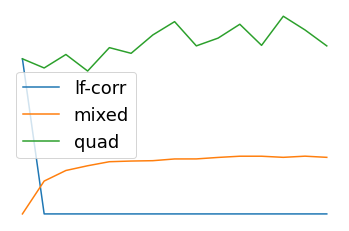
\includegraphics[scale=0.5]{/corr-1000d.png}
% \centering
% \caption{Зависимость итоговой стоимости от коэффициента k, 1000\$/кВт ч}
% \label{fig:corr-1000}
% \end{figure}

% \begin{figure}[h]
% 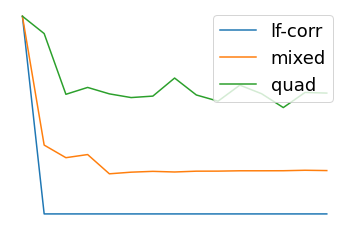
\includegraphics[scale=0.5]{/corr-400d.png}
% \centering
% \caption{Зависимость итоговой стоимости от коэффициента k, 400\$/кВт ч}
% \label{fig:corr-400}
% \end{figure}

% \begin{figure}[h]
% 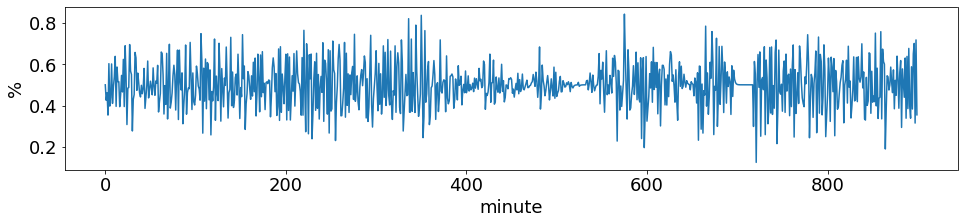
\includegraphics[scale=0.5]{/core.png}
% \centering
% \caption{График изменения заряда опорной батареи}
% \label{fig:core}
% \end{figure}


\subsection{Обзор продвинутых методов решения задачи планирования}

\begin{itemize}
    \item Учет нелинейностей \\
    Учёт нелинейности топливной характеристики дизель-генератора,
    зависимости износа батареи от глубины и тока заряда/разряда.
    В таком случае могут быть вычислительные проблемы с поиском точного решения методами выпуклой оптимизации.
    Применяются эвристические алгоритмы оптимизации, такие как алгоритм светлячка \cite{Sufyan2019}.
    
    \item Методы искусственного интеллекта\\
    Повышенный интерес к искусственному интеллекту и машинному обучению вкупе со сложностью поиска глобально-оптимальных решений в явном виде, приводит к существованию большого разнообразия подходов на основе методов искусственного интеллекта, например, генетических алгоритмов, нечёткой логики и полносвязных нейронных сетей \cite{Olatomiwa2016, kerdphol2016rbf, chaouachi2012multiobjective, jafari2018adaptive}.
    
    \item Model predictive control \\
    Хотя в литературе есть результаты, показывающие, что простые стратегии управления в некоторых случаях могут давать глобально-оптимальные решения \cite{Barley1996}, представляет интерес поиск универсальных глобально-оптимальных алгоритмов управления.
    Один из подходов, в которых явно заложен учёт оптимальности работы системы на следующих итерациях --- использование модельно-прогностического управления (Model Predictive Control, MPC).
    В статье \cite{Tazvinga2014} целевая функция MPC была составлена таким образом, чтобы минимизировать использование дизель-генератора и максимизировать использование ВИЭ; 
    было показано, что при наличии ошибок в прогнозировании потребления и генерации ВИЭ управление с помощью MPC на тестовой модели эффективнее управления с помощью квадратичного программирования (аналогично сформулированной выше задаче MILP для LF (\ref{f:lf}), только функция расхода дизеля имеет вид $aP^2 + bP$).
    
    \item Стохастическая оптимизация
    
    
    Пожалуй, в наиболее общем виде задача оптимального управления микрогридом может быть записана как задача минимизации матожидания затрат на эксплутацию системы на нескольких следующих периодах, то есть как задача стохастической оптимизации:
    \begin{equation}
        \E\left( \sum_{k=0}^m c_k ~\vert~ u_0 \right) \rightarrow \min\limits_{u_0},
    \end{equation}
    
    где $c_k$ --- затраты на $k$-ом интервале планирования, случайная величина, зависящая от вероятностных распределений случайных процессов ветрогенерации и нагрузки; $u_0$~--- управление на ближайший интервал.
    
    % Частными случаями такого подхода являются стратегии $CC$ и $LF$ --- при ветрогенерации равной нулю или достаточно большой константе соответственно.
    
    В статье Zeng P. et al. \cite{zeng2018dynamic} задача управления микрогридом в форме стохастической оптимизации решается методом приближенного динамического программирования (Approximate dynamic programming, ADP) с помощью рекуррентных нейронных сетей (Reccurent neural network, RNN).
    
    
    % \item Оперативная коррекция\\
    % Учёт возможности изменения нагрузки и ветрогенерации после планирования. 
    % Простейшее решение --- добавить в задачу оптимизации условие на наличие резерва мощности, доступного без включения на этапе оперативной коррекции новых генераторов.
    % При анализе решений задачи планирования для оценки эффективности по этому параметру (\textit{reliability analysis}) оценивают вероятность нехватки мощности \cite[8]{Sufyan2019} или вносят условие на её максимальное значение в ограничения оптимизационной задачи \cite[5]{Petersen2018}.
    
    \item Баланс реактивной мощности и задача об оптимальном потоке мощности\\
    При анализе физических процессов в системе мы ограничились уравнением баланса активной мощности, считая, что реактивная мощность в потреблении незначительна, и что физические соединения спроектированы таким образом, что мы можем не думать об ограничениях и потерях мощности в линиях.
    При необходимости, можно обратить внимание на баланс реактивной мощности \cite{zhang2016reactive} или рассмотреть более общую постановку задачи на основе уравнений потока мощности в сети \cite{kim2000comparison, molzahn2017survey}.
    
\end{itemize}
